\documentclass[12pt]{article} 

\usepackage[a4paper,
            bindingoffset=0.2in,
            left=0.75in,
            right=0.52in,
            top=0.75in,
            bottom=1.44in,
            footskip=.25in]{geometry}

\usepackage{graphicx}
\graphicspath{ {./image/} }

\usepackage{array}
{\renewcommand{\arraystretch}{2}% for the vertical padding

\usepackage{parskip}
\setlength{\parindent}{0pt}

\setcounter{secnumdepth}{0}

\title{Epidemic Modelling SIR Model}
\author{Amrit Baral, , Nabin Da Shrestha, Nirajan Bekoju, Nishant Luitel}
\date{August 23, 2022} 

\begin{document}  

\bigskip
\bigskip
\bigskip
\bigskip

\begin{center}

\includegraphics[scale = 0.5]{logo.png}

Tribhuwan University

Institute of Engineering

Pulchowk Campus

\bigskip
\bigskip
\bigskip
\bigskip

\noindent\makebox[\linewidth]
{\rule{15cm}{0.4pt}}
A Project Report on:

\textbf{\large Volunteer Management System}
\noindent\makebox[\linewidth]
{\rule{15cm}{0.4pt}}

\bigskip
\bigskip
\bigskip
\bigskip
\textbf{Submitted By:}

Amrit Baral(076bct006)

Nabin Da Shrestha(076bct037)

Nirajan Bekoju(076bct039)

Nishant Luitel (076bct041)

\bigskip
\bigskip
\bigskip
\bigskip
\textbf{Submitted To:}

Department of Electronics and Computer Engineering

\bigskip
\bigskip
\bigskip
\bigskip
\textbf{Submission Date:} 

25th August, 2022

\end{center}



\clearpage

\section{Acknowledgement}
Foremost we want to express our deepest gratitude to our lecturer, Dr. Aman Shakya
for his detailed guidelines for this project. His valuable lectures and lab sessions will be
fundamental cornerstones for this project.

We would like to recognize the enormous influence of past projects from our seniors that gave us
the motivation to come up with this project. Also, our appreciation for all the fellow friends who
have offered us to help in time of need.

We also wish to thank the entire Department of Electronics and Computer Engineering, 
Pulchowk campus for giving students early experience in implementing their own ideas by
working on a real project.

\clearpage

\tableofcontents
\clearpage

\section{Abstract}
A volunteer management system is a software created to help organizations adminster volunteer programs, events, or initiatives. This software offers volunteer recruitements features, scheduling, management and communication and acts as a database for all of an organization's volunteer information. This software also offers feature sets specifically fo the administrative requirements to manage any number of volunteers and events. Volunteer Management System ensure the sustainability of any programs and events that rely on volunteer's work. In short, Volunteeer management system can make sure that the any events that an organization perform has enough number of volunteers and also promote volunteering. All the events of the organization can be managed and scheduled and event manager can invite volunteer for the upcoming events. 

\textbf{Keywords: } Volunteer Management, Web Development, Django, API, React, DFD 

\clearpage

\section{Introduction}
Volunteering has been one of the most important factor for the successful completion of events. Several task in any events can't be completed without the help of volunteers. However, it is important for any organization to get complete information about volunteers so that they can know whether they are suitable of volunteering in a particular events or not. That is where volunteer management system can help. Because volunteer management system contains all the required information about the volunteer and it also provides a platform for communication between the volunteer and organization where organization can perform some question answering before recruiting the volunteers. Volunteers can also get detail information about the events being organized and they can show interest as well as request to be a volunteer in out proposed system.

\subsection{Problem Statement}
Recruiting right volunteers for an event is an important factor as skillset of volunteer matters in the smooth coordination in any event. Organizations have trouble to inform volunteer about the upcoming events and to check if volunteers are available for the event or not. It is difficult for any organization to guess the number of volunteers available and their needs as well. Moreover, it might be tedious for volunteers to apply physically. So, volunteer management system's goal is to solve all these problems and it is built with following objectives.

\subsection{Objectives}
\begin{itemize}
	\item To manage all the events of an organization.
	\item To provide a platform for communication between volunteer and event manager.
	\item To verify the qualifications of volunteer for an event.
	\item To promote volunteering
\end{itemize}

\clearpage
\clearpage

\section{Programmer's Guide}
\subsection{Software Detail}
\begin{enumerate}
	\item Technical Detail of Implementation
	
	Volunteer management system was built using Dango and  Django Rest Framework for backend and React, Redux for Frontend. Sqlite was used as database in local server but PostgreSQL was used while hosting the website. 	
	
	\item Authentication Detail
	
	Json Web Token Authentication was used with the help of djangorestframework-simplejwt version 4.7.2.
	
	\item Level 0 Data Flow Diagram
	
	Level 0 Data Flow Diagram shows the flow of data from volunteer, admin and organization to and from the volunteer management system. All the functional features are shown briefly in the given level 0 data flow diagram.	
	
	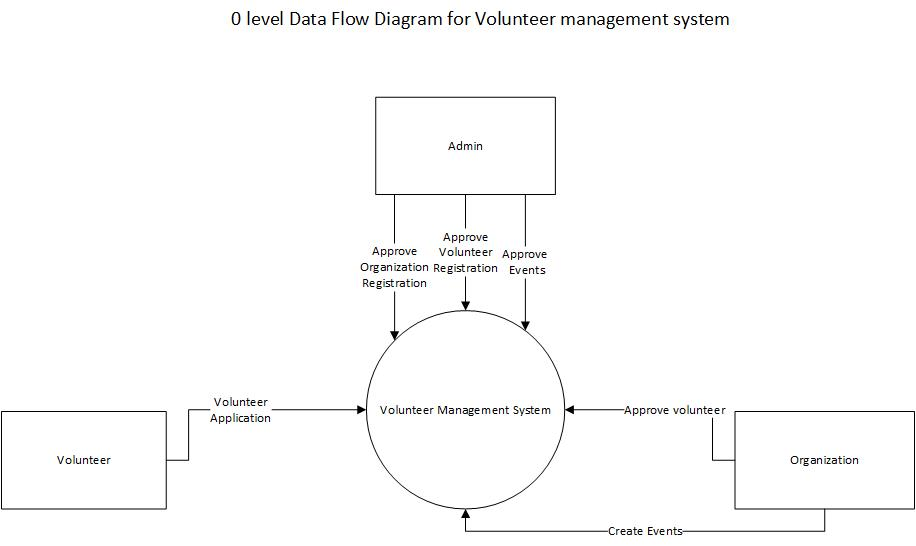
\includegraphics[scale = 0.85]{DFD0.jpg}


\clearpage
\clearpage

	\item Level 1 Data Flow Diagram
	
	Level 1 data flow diagram shows all the description of how data flow occurs in volunteer management system and detail action of organization, volunteer and admin of this system. It shows all the related process as well as the database table and data flow between them in detail. 
			
	\begin{center}
	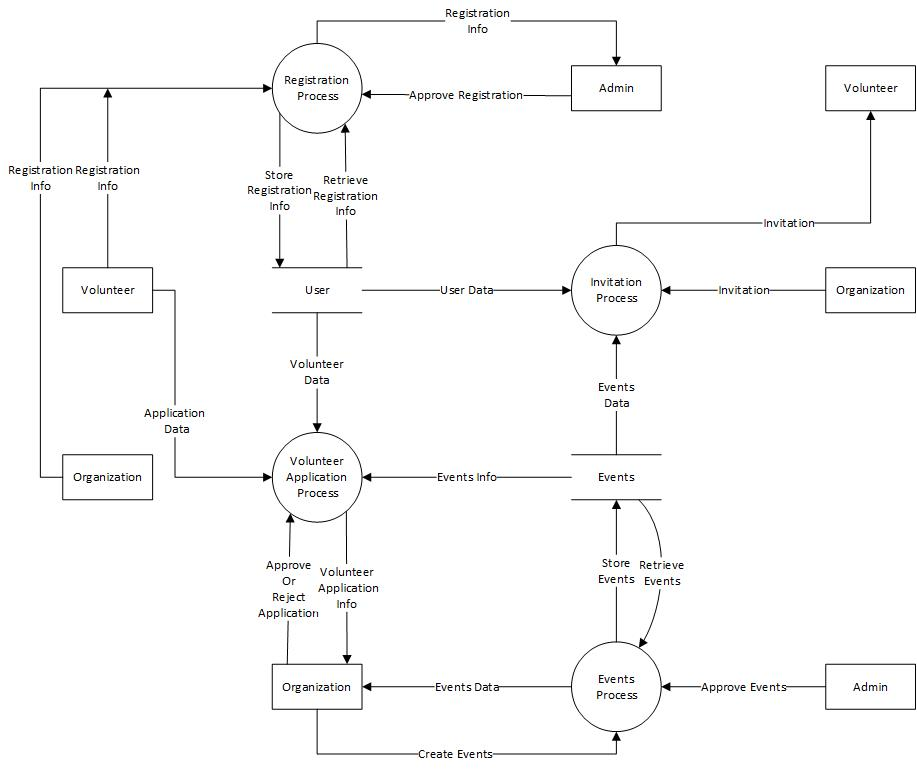
\includegraphics[scale = 0.8]{DFD1.jpg}
	\end{center}	
		
	\clearpage
	\clearpage

	\item Entity-Relationship Diagram
	
	Following diagram shows the entity-relationship diagram of the volunteer management system.
	
	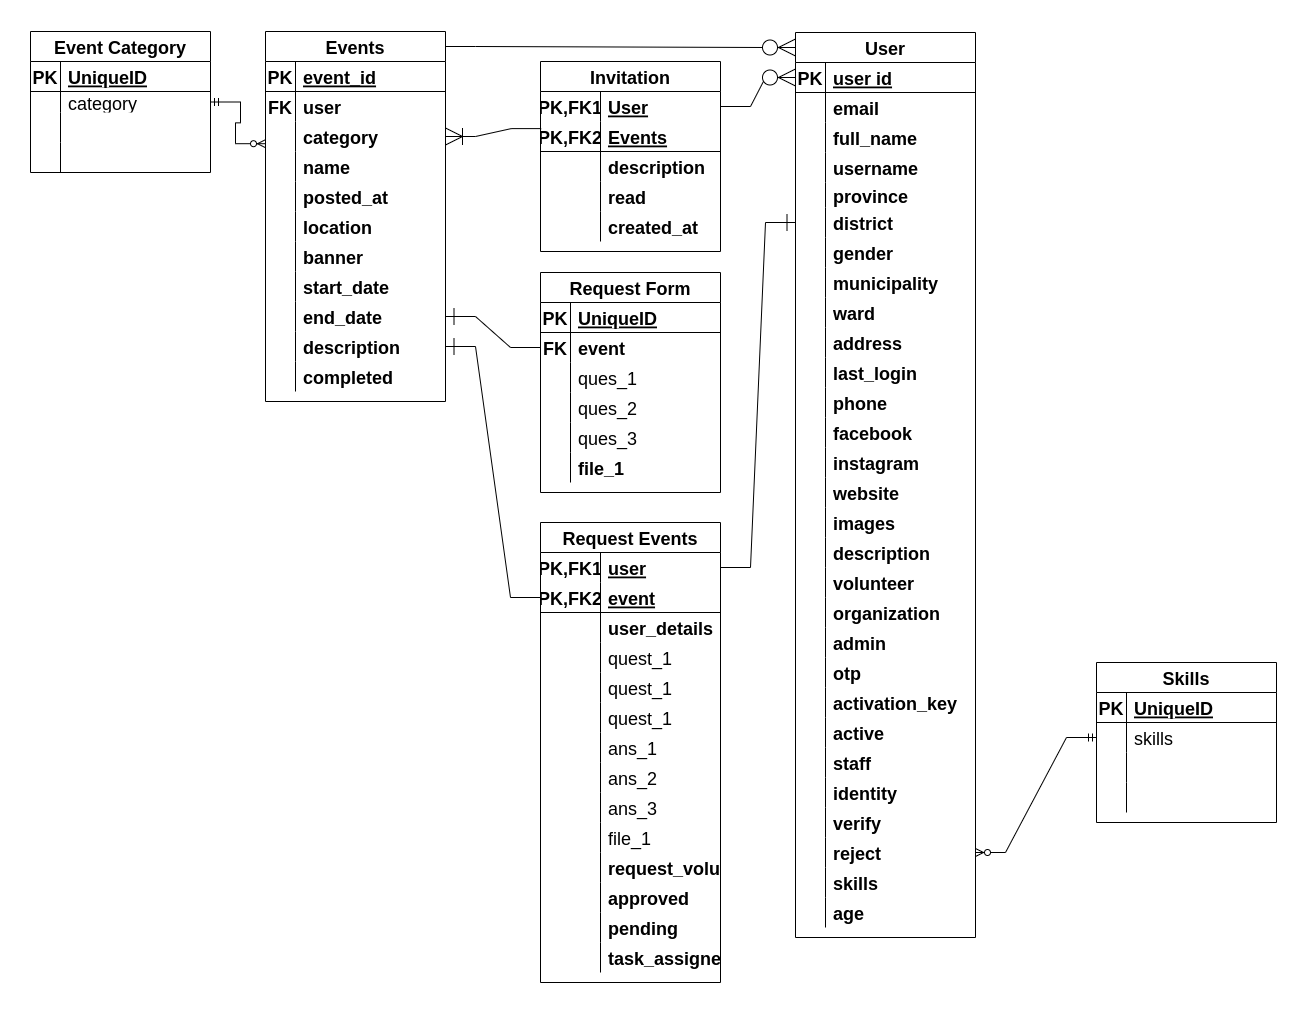
\includegraphics[scale = 0.35]{ER1.png}

\end{enumerate}

\clearpage
\clearpage

\subsection{API Endpoints Details}
Api Documentation was made with the help of Swagger. A brief details of all api grouped into django application are given below:

\begin{enumerate}
	\item Authentication
	
	This application deals with all the authentication works like login, logout, profile detail and password reset.

	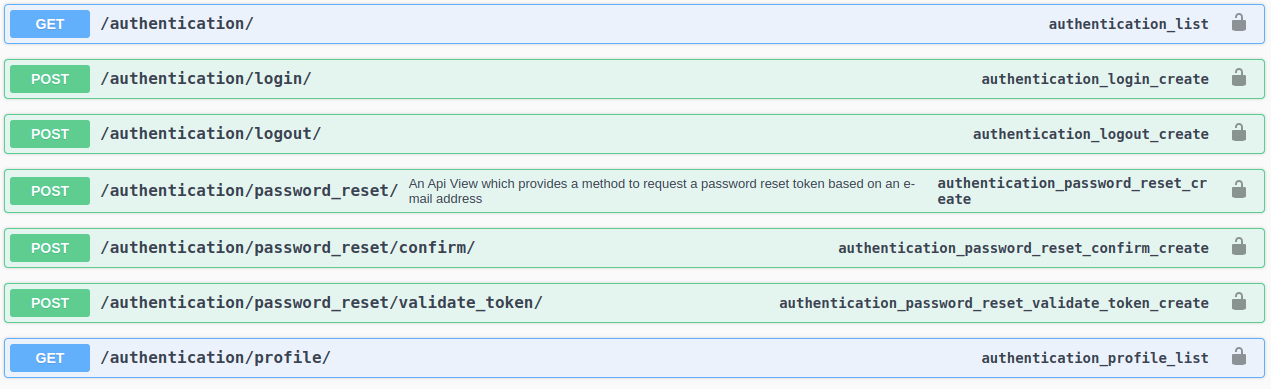
\includegraphics[scale = 0.35]{auth.png}			
	
	\item Category
	
	This app contains all the information about the category of the events and skills of the volunteers.	
	
	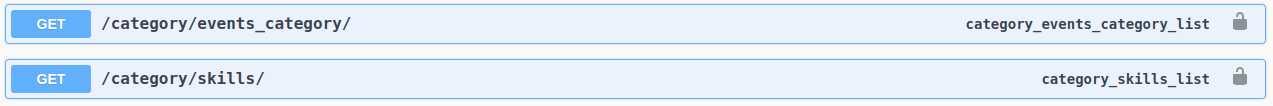
\includegraphics[scale = 0.35]{category.png}	
	
	\item Events
	
	This app contains all the information about events management such as events history, events registration, update and deletion.
	
	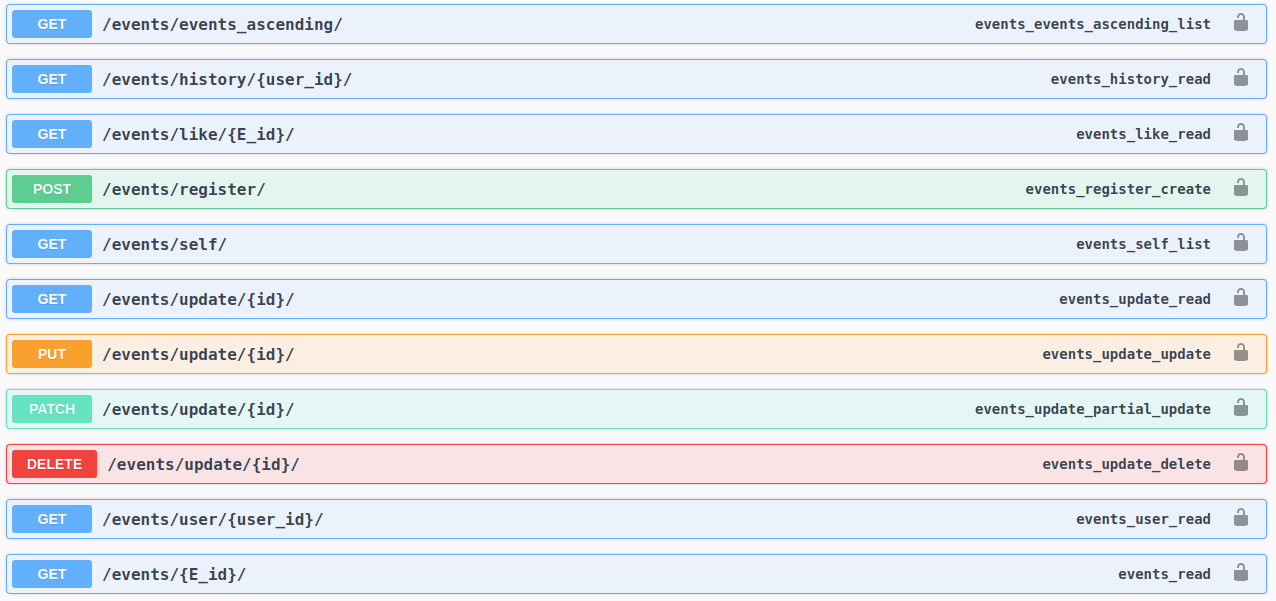
\includegraphics[scale = 0.35]{events.png}		

\clearpage
\clearpage

	\item Invite
	
	This app deals with the invitation of the events to volunteers with email features.	
	
	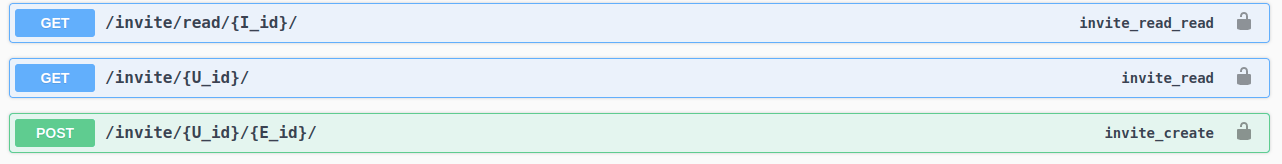
\includegraphics[scale = 0.35]{invite.png}	
	
	\item Miscellaneous
	
	This application handles the basic operation like searching and sorting of events.
	
	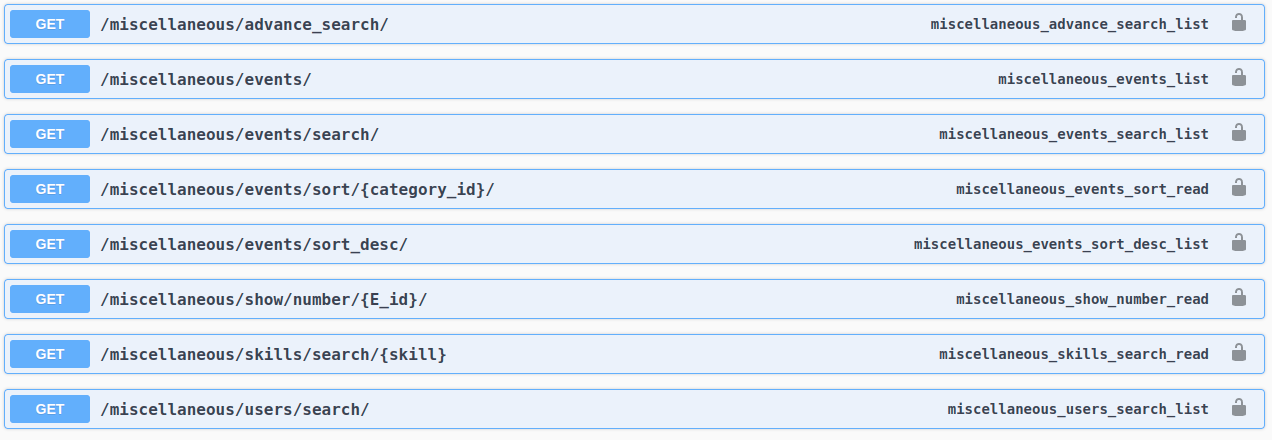
\includegraphics[scale = 0.35]{miscellaneous.png}	
	
	\item Organiation
	
	This application provide the request form to join an event for volunteers and also approve the volunteer request form after the proper review of volunteer detail and question answering.
	
	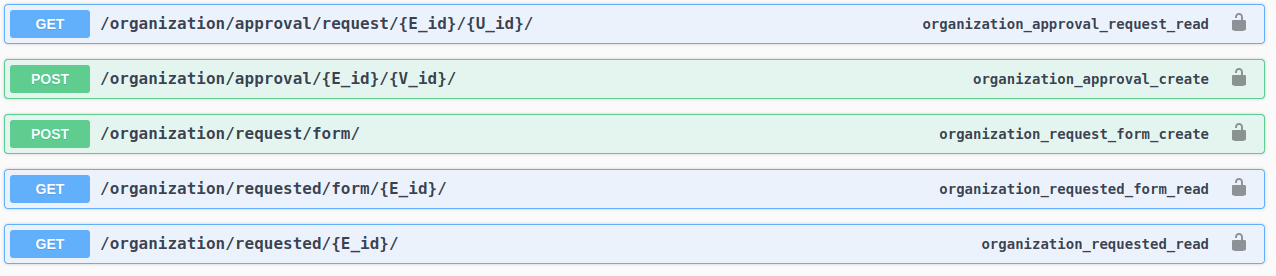
\includegraphics[scale = 0.35]{organization.png}	

\clearpage
\clearpage

	\item User

	This application deals with user registration, profile update and verification.
	
	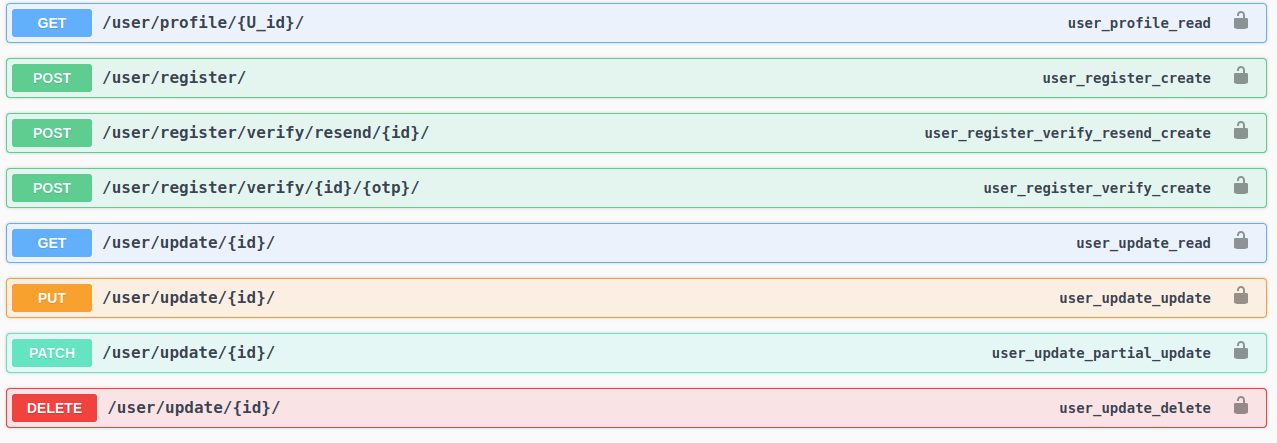
\includegraphics[scale = 0.35]{user.png}	
	
	\item Validate

	This application deals with email validation.	
	
	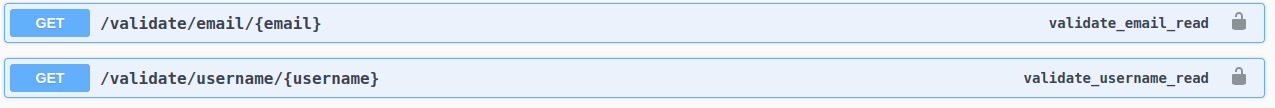
\includegraphics[scale = 0.35]{validate.png}	
	
	\item Verification
	
	This application deals with the verification of volunteer as well as organization by the admin of volunteer management system.
	
	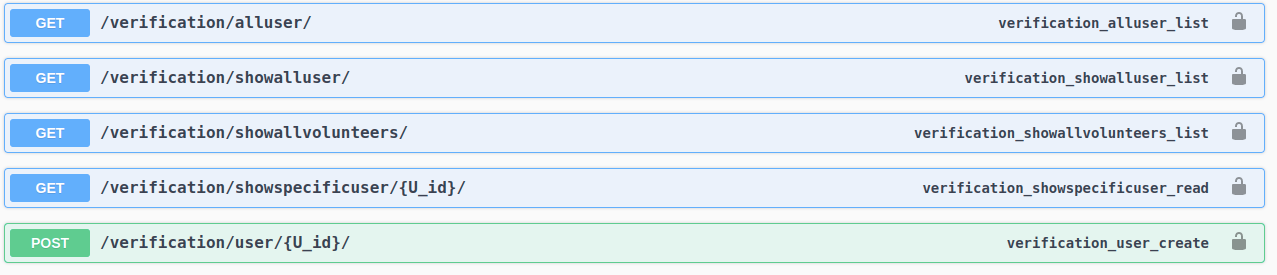
\includegraphics[scale = 0.35]{verification.png}	
	
	\item Volunteer
	
	This application helps volunteer to show interest in an event and apply for specific events along with question answering in the organization's volunteer request form.
	
	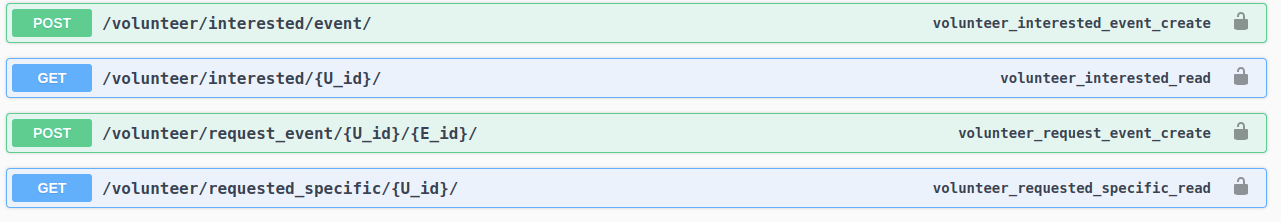
\includegraphics[scale = 0.35]{volunteer.png}	
	
\end{enumerate}

\clearpage
\clearpage

\section{User's Guide}
\subsection{Basic Detail}
\begin{enumerate}
	\item Home Page
	
		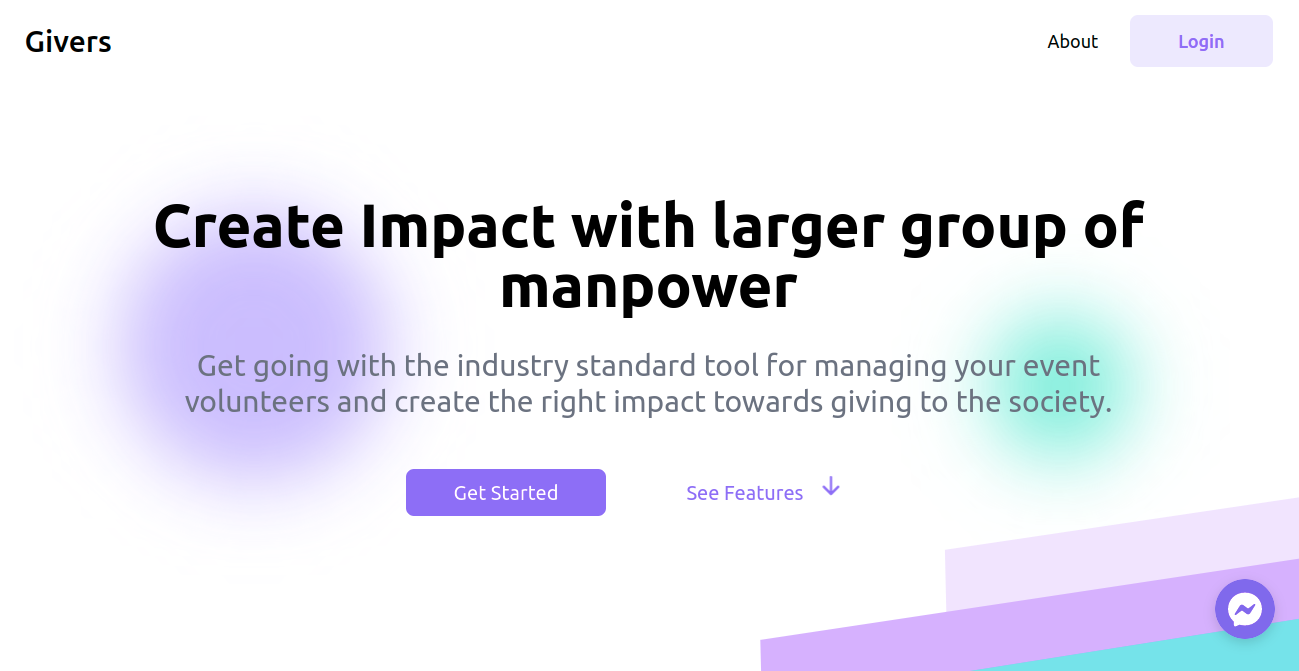
\includegraphics[scale = 0.35]{user/givers_home.png}

		In order to login, click the upper right corner Login Button.

	\item Login

		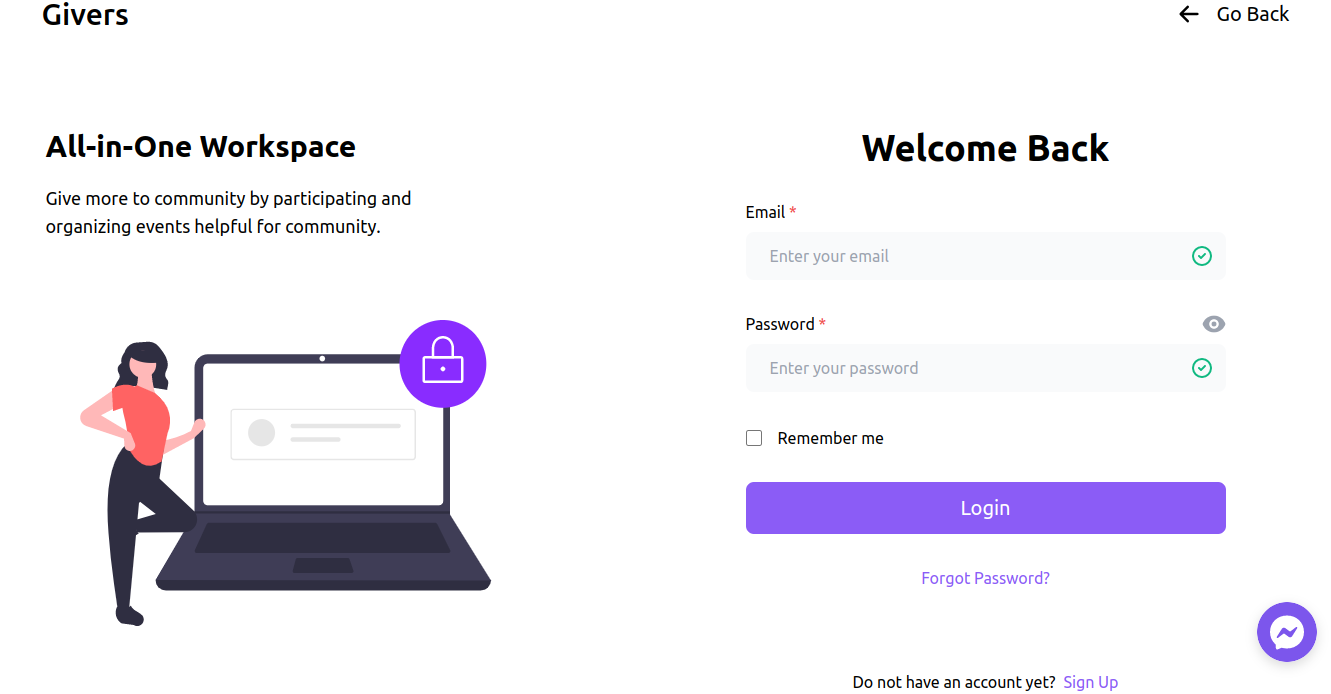
\includegraphics[scale = 0.35]{user/login_page.png}

		This is the login page. You can login and if you donot have an accout, click the sign up link at the bottom of the form.
\clearpage
	\item Registration

		Here, you can register as an organization or a volunteer and follow up five steps to sign up.

		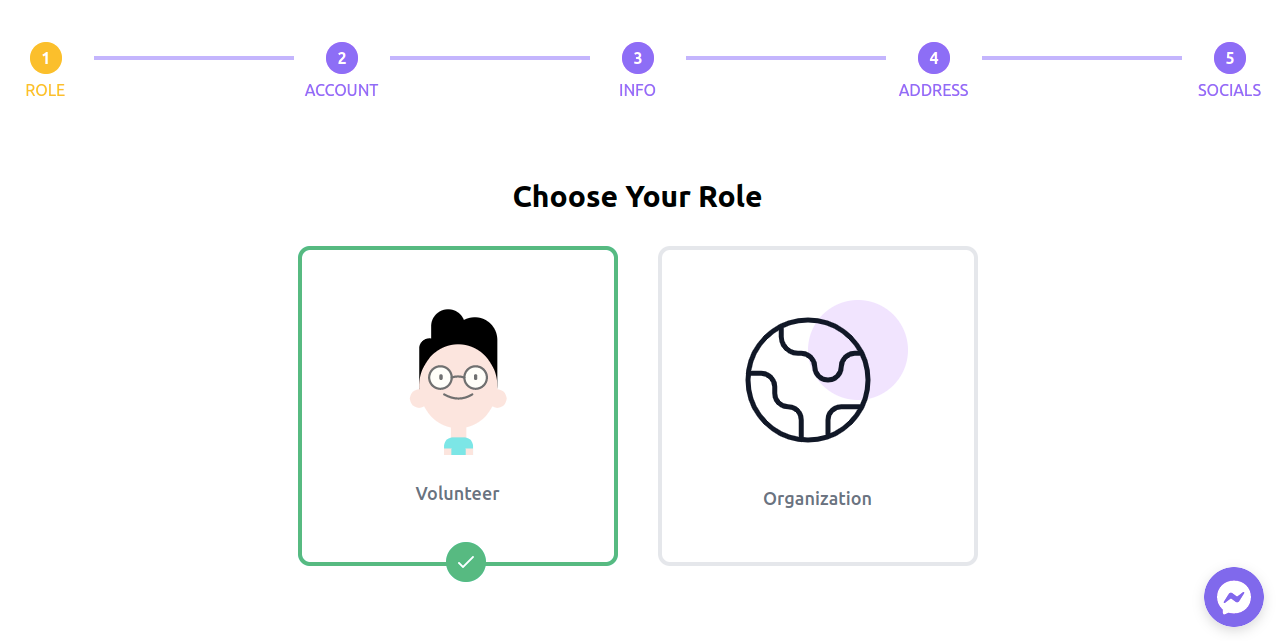
\includegraphics[scale = 0.35]{user/user_register.png}

\end{enumerate}

\clearpage
\clearpage

\subsection{Organiation' Guide}
\begin{enumerate}
	\item Home Page
	
	In the home page, we can see different menu in the left bar and a newsfeed to follow up the events in the middle division.
	
	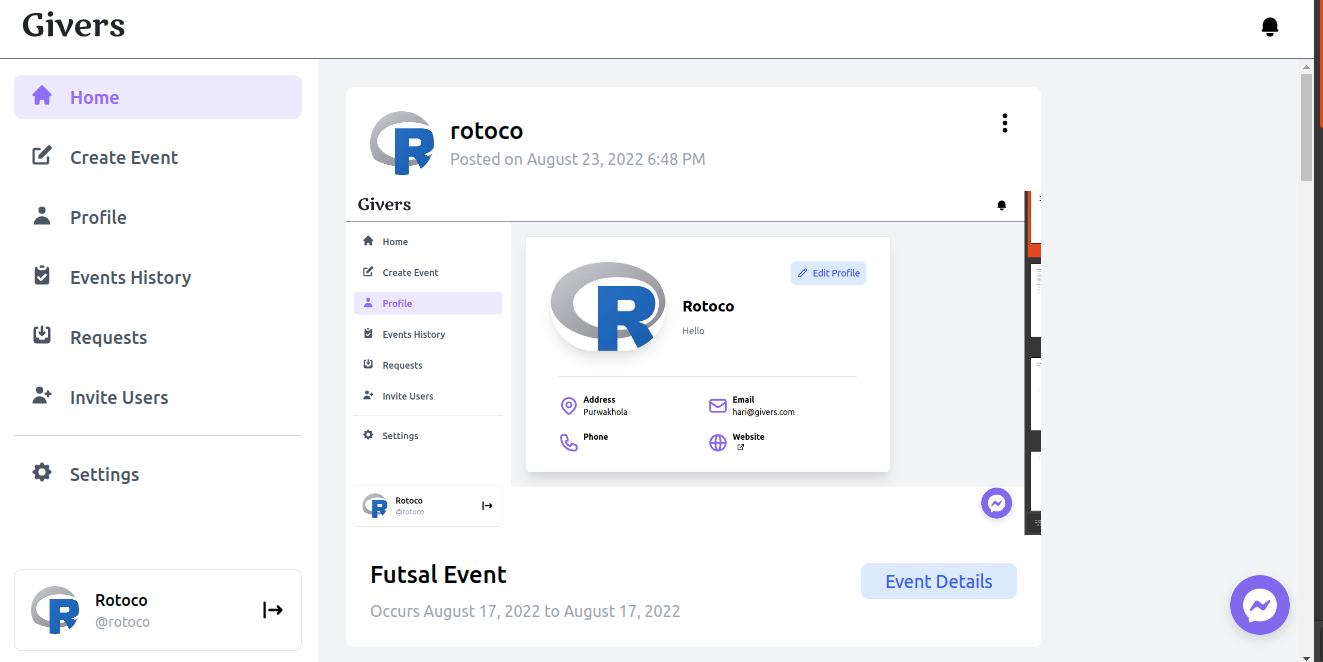
\includegraphics[scale = 0.35]{user/organization_home1.png}

	\item Profile
	
	
	We can view the profile detail as well as edit profile with the help of Edit Profile Button on the upper right corner.
	
	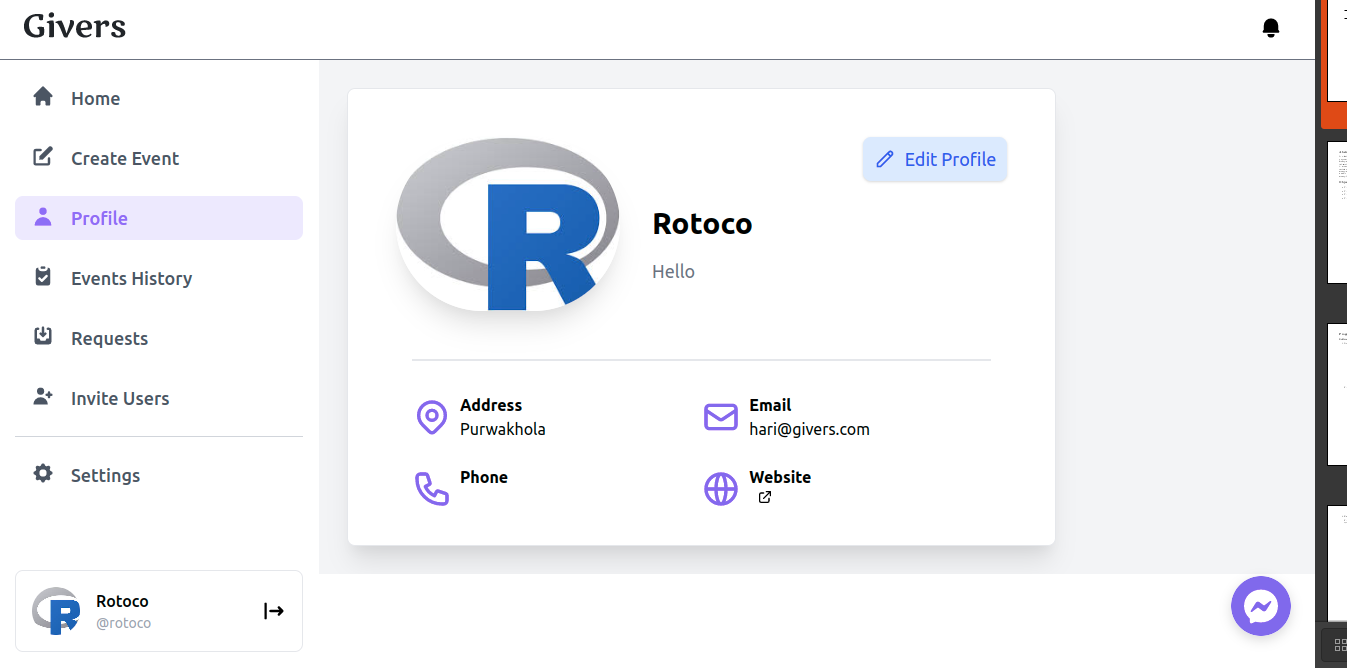
\includegraphics[scale = 0.35]{user/profile_menu.png}

\clearpage

	\item Create Events
	
	Fill up the create event form as shown below to create an event.
	
	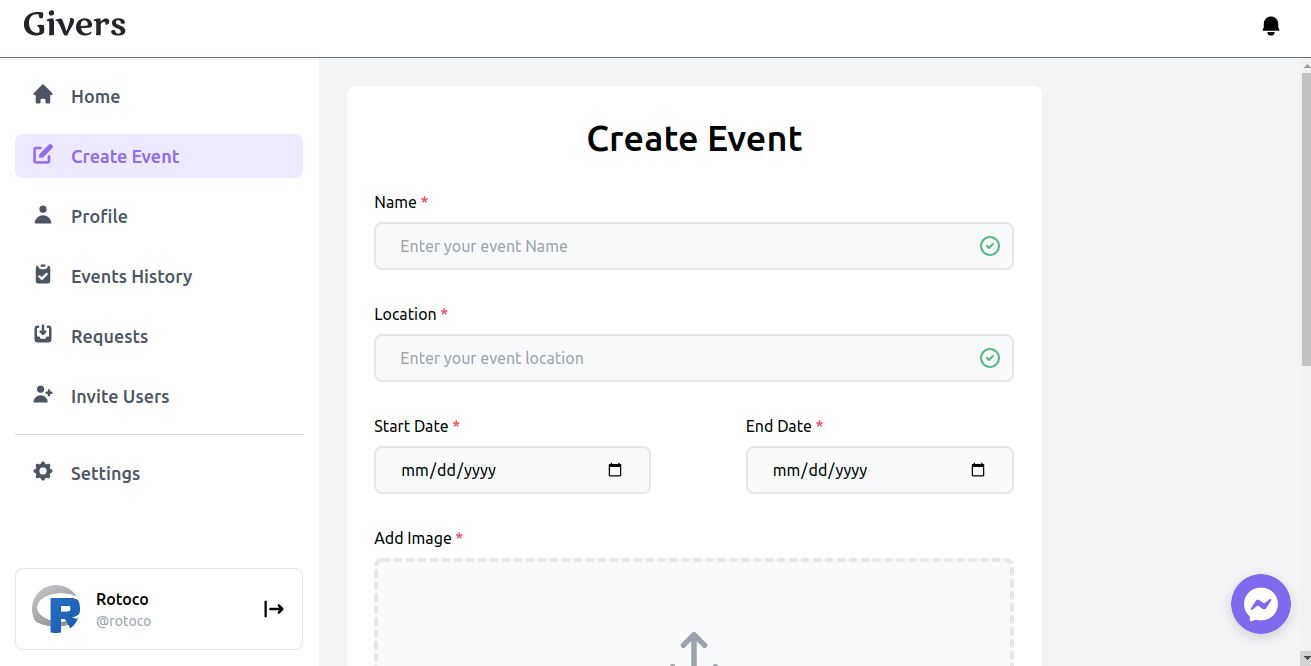
\includegraphics[scale = 0.35]{user/event_creation0.png}

	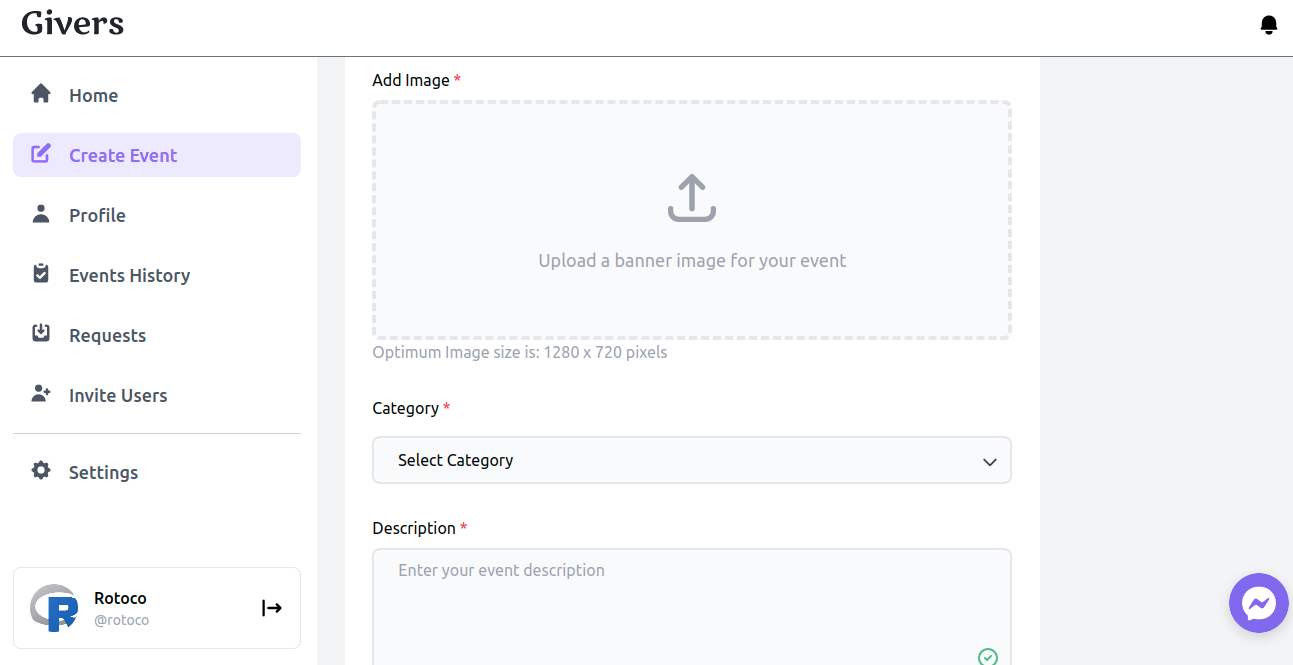
\includegraphics[scale = 0.35]{user/event_create1.png}
	
	\item Event History
	
	This menu contains all the events that the organization has completed.
	
	\item Requests
	
	This menu contails all the events list that the organization has requested volunteers for.
	
	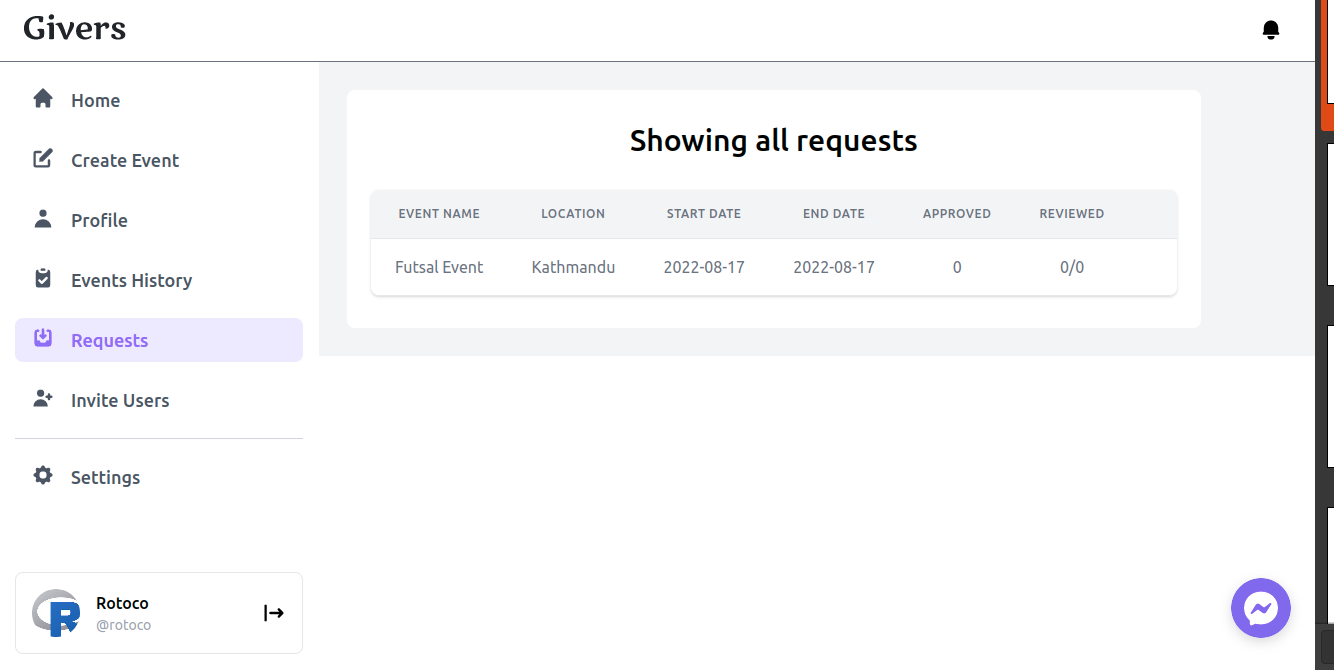
\includegraphics[scale = 0.35]{user/events_request.png}

	\item Invite Users

	This menu shows all the upcoming events and the invited volunteer and participants in the event after clicking View All link.	
	
	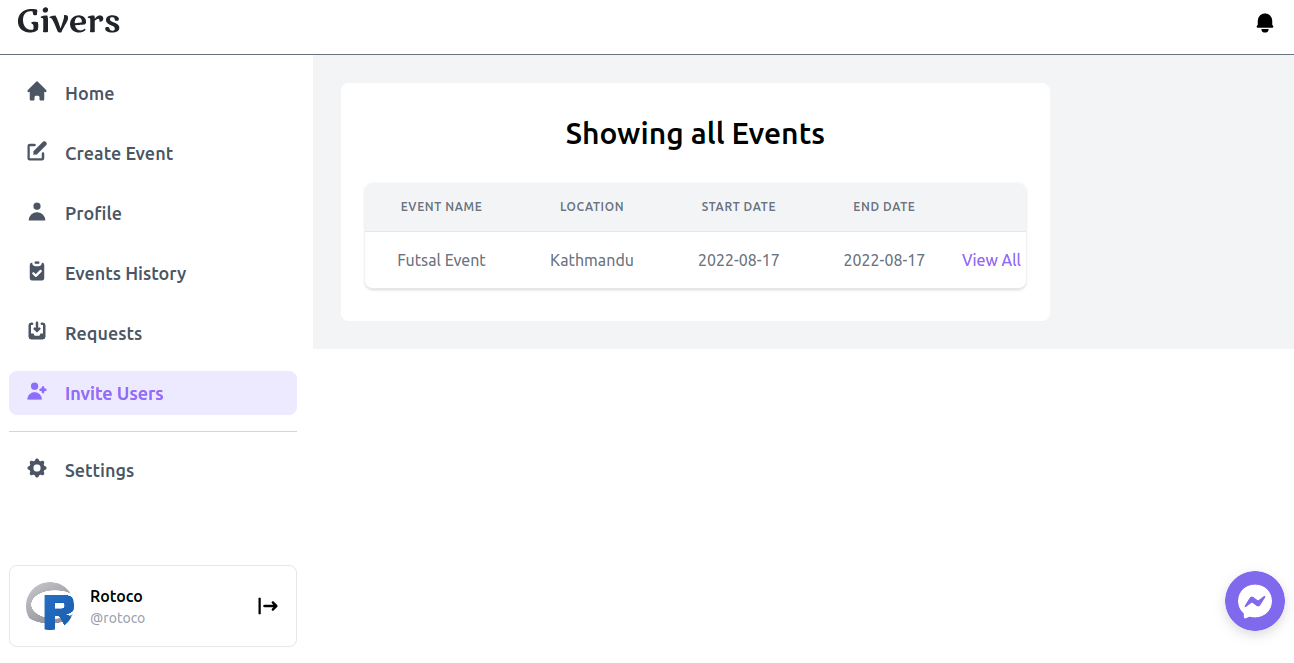
\includegraphics[scale = 0.35]{user/invite_user.png}	
	
	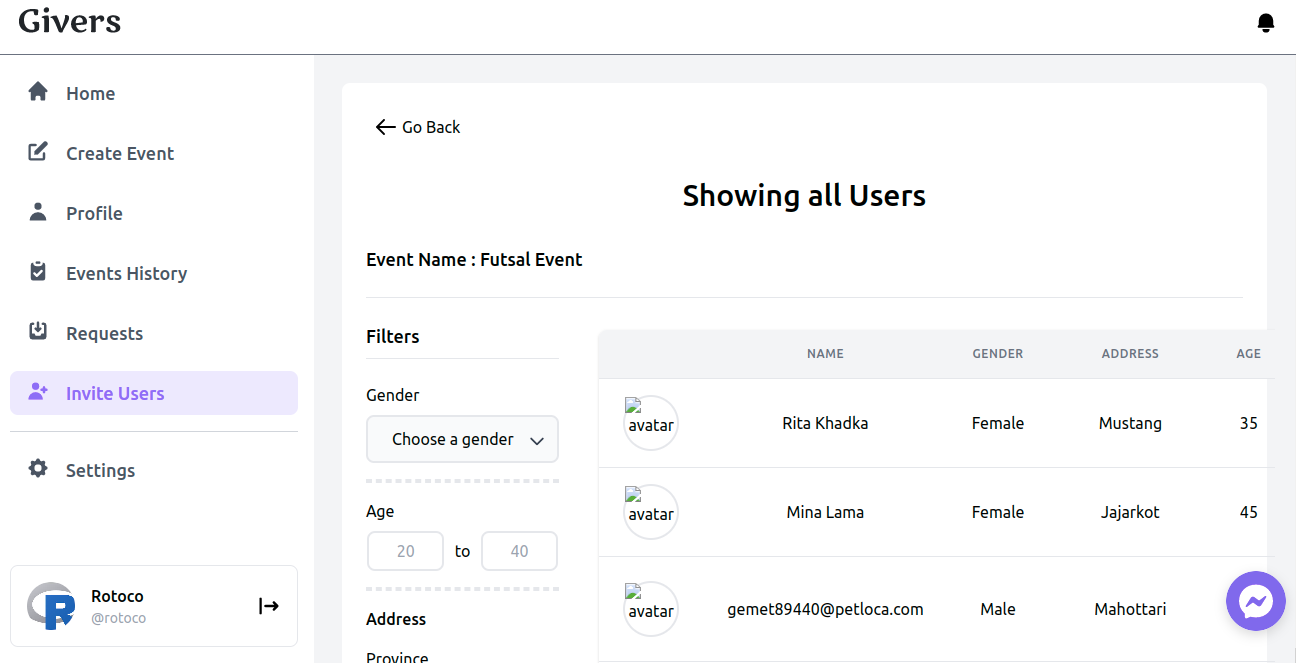
\includegraphics[scale = 0.35]{user/invited_user1.png}
	
\end{enumerate}
	

\clearpage
\clearpage

\subsection{Volunteer's Guide}
\begin{enumerate}
	\item Volunteer Home
	
	This is the home page of the volunteer where we can see the menu on the left bar and newsfeed of upcoming events in mid division. 

	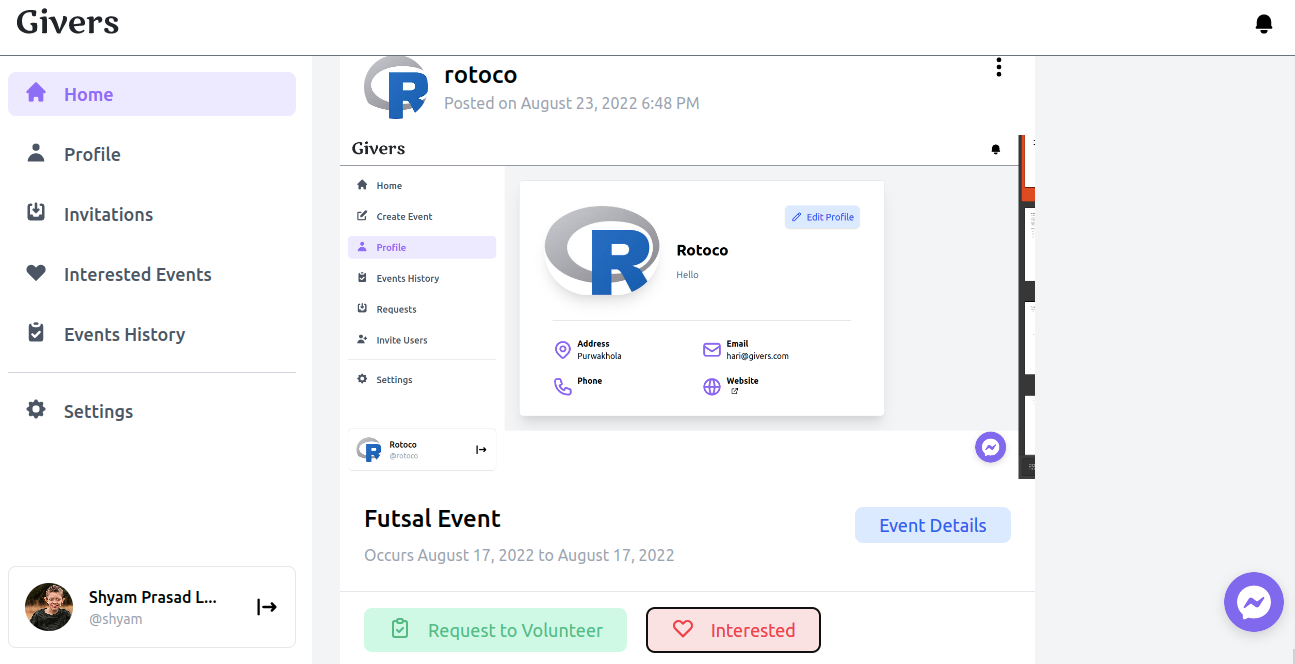
\includegraphics[scale = 0.35]{user/user_home.png}
	
	The events post contains a bar for event detail where volunteer can show interest to an event as well as request to be a volunteer.	
	\begin{center}
	
	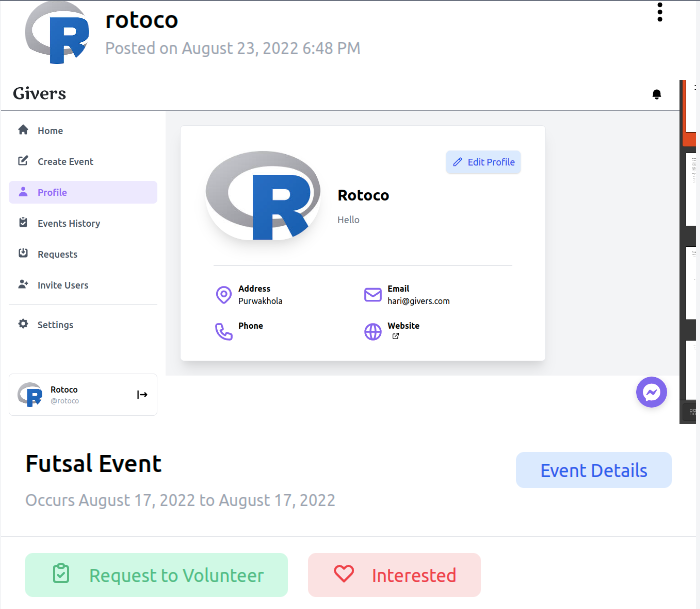
\includegraphics[scale = 0.35]{user/event_post.png}
	
	\end{center}

\clearpage
\clearpage

	\item Profile
	
	Below is the profile menu of Volunteers where they can see the detail as well as edit profile.
	
	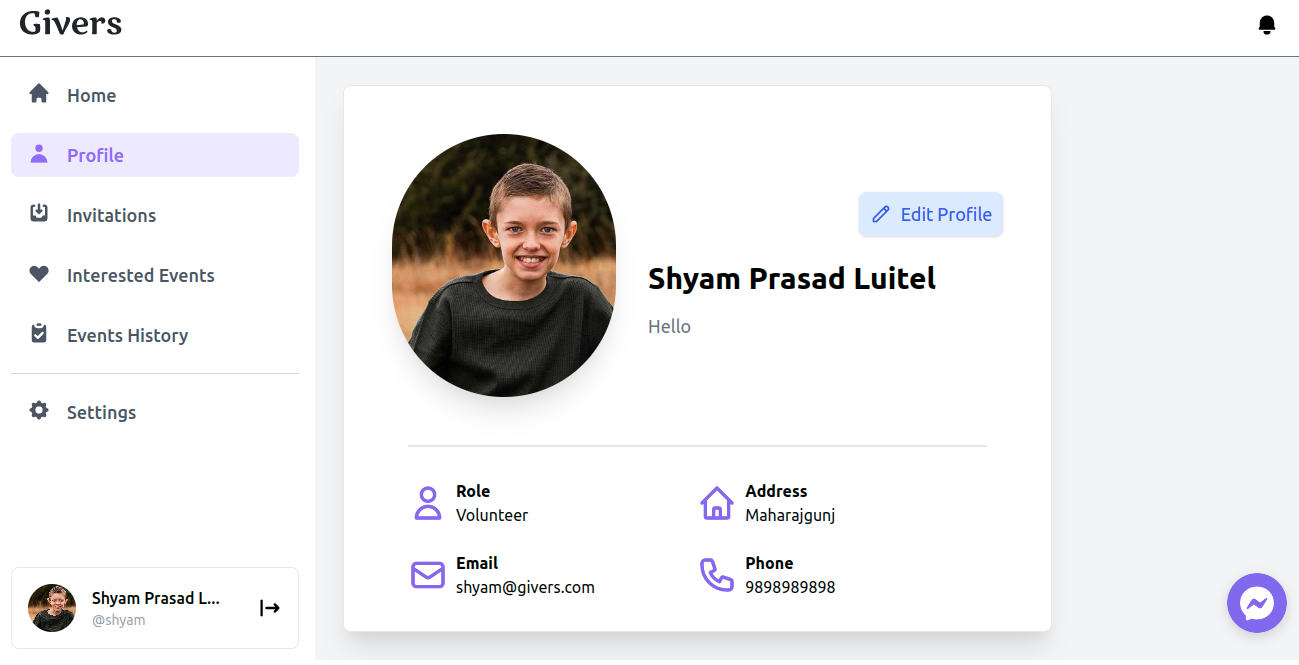
\includegraphics[scale = 0.35]{user/user_profile.png}		
	
	\item Invitations
	 
	This menu contains all the invitations from organizations for an event.
	
	\item Interested Events
	
	This menu shows all the events that the volunteer is interested in.
	
	\item Events History
	
	This meny shows all the events that the volunteer has participated.
	
\end{enumerate}

\clearpage
\clearpage

\section{Conclusion}
Volunteers play significant role in the successful completion of any events of any organization. With the help of volunteer management system, any registered organization are able to manage events and request for volunteers on the basis of certain skillsets and question answering. Validation of volunteer skills and approval of request form is possible through this system. Moreover, Volunteer can also search for the events which are more likely of their interests and can contribute and also develop self personality. In summary volunteer management system provides platform to organization and volunteer for the successful execution of any program.

\section{Future Enhancement}
\begin{enumerate}
	\item In order to promote volunteering work, Badge will be provided to the volunteers.
	\item Review of events and volunteering experience platform will be added.
	\item Availability of volunteer feature will be added.
	\item For the effective communication between organization and volunteer, real time chat features will be added. 
\end{enumerate}




\end{document}